\hypertarget{iiot-e-tecnologias-emergentes}{%
\chapter{IIoT e Tecnologias Emergentes}\label{iiot-e-tecnologias-emergentes}}

\section*{Objetivos de Aprendizagem}

Ao final deste capítulo, o leitor será capaz de:

\begin{itemize}
\tightlist
\item
  Distinguir IoT de IIoT e compreender seus requisitos industriais específicos.
\item
  Descrever as arquiteturas de Edge, Fog e Cloud Computing e seu papel na automação.
\item
  Compreender o conceito de Digital Twin e suas aplicações industriais.
\item
  Identificar ferramentas de análise de dados industriais (Grafana, InfluxDB, Kafka).
\end{itemize}

\begin{center}\rule{0.5\linewidth}{0.5pt}\end{center}

\hypertarget{iot-versus-iiot}{%
\section{IoT versus IIoT}\label{iot-versus-iiot}}

A \textbf{IoT} (\emph{Internet of Things} --- Internet das Coisas) é o paradigma em que objetos físicos são conectados à internet, coletando e trocando dados. Aplicações populares: termostatos inteligentes, câmeras de segurança, rastreadores de fitness.

O \textbf{IIoT} (\emph{Industrial Internet of Things} --- Internet Industrial das Coisas) aplica esses conceitos ao ambiente industrial, mas com requisitos muito mais rigorosos:

\textbf{Tabela 6.1 -- IoT \ensuremath{\times} IIoT: principais diferenças}

\begin{longtable}[]{@{}
  >{\raggedright\arraybackslash}p{(\columnwidth - 4\tabcolsep) * \real{0.3333}}
  >{\raggedright\arraybackslash}p{(\columnwidth - 4\tabcolsep) * \real{0.3333}}
  >{\raggedright\arraybackslash}p{(\columnwidth - 4\tabcolsep) * \real{0.3333}}@{}}
\toprule\noalign{}
\begin{minipage}[b]{\linewidth}\raggedright
Critério
\end{minipage} & \begin{minipage}[b]{\linewidth}\raggedright
IoT (Consumidor)
\end{minipage} & \begin{minipage}[b]{\linewidth}\raggedright
IIoT (Industrial)
\end{minipage} \\
\midrule\noalign{}
\endhead
\bottomrule\noalign{}
\endlastfoot
\textbf{Confiabilidade} & Tolerável falha ocasional & Falha pode causar acidente ou parada de planta \\
\textbf{Latência} & Segundos a minutos & Milissegundos a segundos \\
\textbf{Ciclo de vida} & 3--5 anos & 15--30 anos \\
\textbf{Ambiente} & Ambientes domésticos & Calor, vibração, poeira, EMI, atmosfera explosiva \\
\textbf{Segurança} & Importante & Crítica --- sistemas de segurança funcional \\
\textbf{Integração} & App + nuvem & CLP + SCADA + MES + ERP \\
\textbf{Protocolos} & HTTP, CoAP, MQTT, BLE & MQTT, OPC UA, Modbus, DNP3, Sparkplug B \\
\textbf{Normas} & ETSI, IEEE & IEC 62443, ISA-99, IEC 61508 \\
\end{longtable}

\begin{caixafigura}

\textbf{{[}Figura 6.1 -- IoT versus IIoT: ambientes e requisitos{]}}
\emph{Duas ilustrações lado a lado: (esquerda) casa inteligente com dispositivos IoT consumidor (termostato, lâmpada, câmera, smartwatch); (direita) planta industrial com sensores IIoT, gateway de borda, CLP e servidor SCADA. Destacar os requisitos distintos: segurança, latência, robustez.}

\end{caixafigura}

\begin{center}\rule{0.5\linewidth}{0.5pt}\end{center}

\hypertarget{arquitetura-iiot-edge-fog-e-cloud}{%
\section{Arquitetura IIoT: Edge, Fog e Cloud}\label{arquitetura-iiot-edge-fog-e-cloud}}

A arquitetura IIoT é tipicamente organizada em três camadas:

\begin{center}
\IfFileExists{../figuras/capitulo-06-m1.pdf}{%
  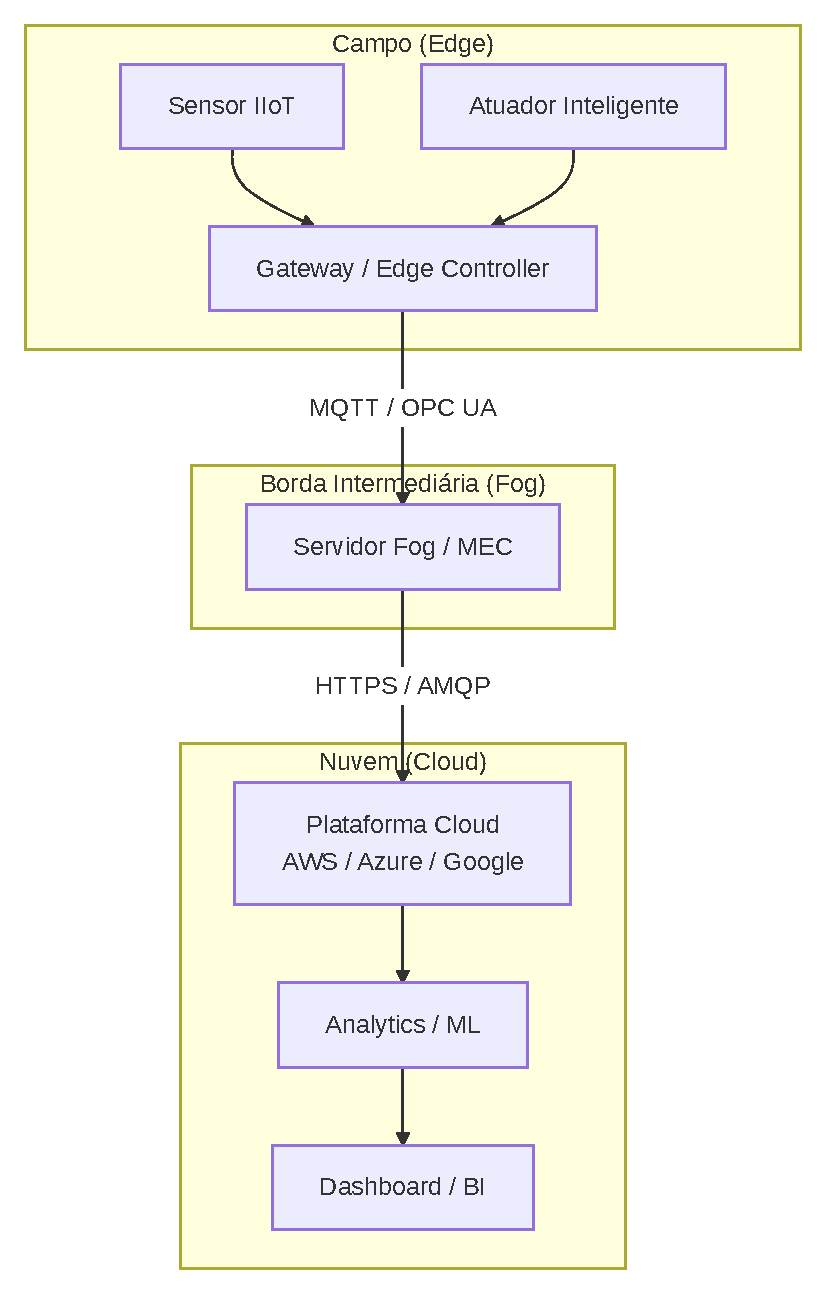
\includegraphics[width=\linewidth,height=0.8\textheight,keepaspectratio]{../figuras/capitulo-06-m1.pdf}%
}{\fbox{\parbox{0.9\linewidth}{\small Diagrama Mermaid ainda não renderizado: capitulo-06-m1. Rode scripts/render-mermaid.sh.}}}
\end{center}

\begin{caixafigura}

\textbf{{[}Figura 6.2 -- Arquitetura IIoT em três camadas: Edge, Fog e Cloud{]}}
\emph{Diagrama em camadas horizontais com ícones: campo industrial (sensores, CLPs, RTUs) na base; gateway/edge controller no meio; e a nuvem no topo com plataformas AWS IoT, Azure IoT Hub e ferramentas de analytics. Indicar os protocolos em cada enlace.}

\end{caixafigura}

\hypertarget{edge-computing}{%
\subsection{Edge Computing}\label{edge-computing}}

O \textbf{Edge Computing} (computação na borda) leva o processamento o mais próximo possível da fonte de dados --- no próprio equipamento ou em um gateway de campo.

\textbf{Por que processar na borda?}
- \textbf{Latência:} ações de controle críticas não podem esperar a nuvem (viagem de ida e volta \textasciitilde100 ms).
- \textbf{Largura de banda:} pré-processar e filtrar dados na borda reduz drasticamente o volume a ser transmitido à nuvem.
- \textbf{Operação offline:} o sistema continua funcionando mesmo sem conectividade com a nuvem.
- \textbf{Privacidade:} dados sensíveis de produção não precisam sair da planta.

\textbf{Exemplos de edge devices:}
- \textbf{Gateways industriais:} Moxa UC-8100, Advantech UNO-2372G, Siemens SIMATIC IPC.
- \textbf{Edge controllers:} PLCnext (Phoenix Contact), Bedrock Automation, Beckhoff C6015.
- \textbf{Microprocessadores embarcados:} Raspberry Pi (prototipagem), NVIDIA Jetson (IA na borda).

\begin{caixadica}

\textbf{Dica:} O \textbf{AWS IoT Greengrass} e o \textbf{Azure IoT Edge} são plataformas de software que transformam um gateway industrial em um nó de computação inteligente --- executando funções Lambda/containers localmente, com sincronização automática com a nuvem quando conectado.

\end{caixadica}

\hypertarget{fog-computing}{%
\subsection{Fog Computing}\label{fog-computing}}

O \textbf{Fog Computing} adiciona uma camada intermediária entre o edge e a nuvem --- geralmente um servidor instalado na subestação, sala de controle da planta ou datacenter de borda (\emph{MEC --- Mobile Edge Computing}).

\textbf{Funções do Fog:}
- Agregação de dados de múltiplos gateways de campo.
- Processamento de analytics local (detecção de anomalias, correlação de eventos).
- Cache de dados para resiliência a falhas de conectividade WAN.

\begin{center}\rule{0.5\linewidth}{0.5pt}\end{center}

\hypertarget{plataformas-iiot-em-nuvem}{%
\section{Plataformas IIoT em Nuvem}\label{plataformas-iiot-em-nuvem}}

As principais plataformas de nuvem oferecem serviços especializados para IIoT:

\textbf{Tabela 6.2 -- Plataformas cloud para IIoT}

\begin{longtable}[]{@{}
  >{\raggedright\arraybackslash}p{(\columnwidth - 6\tabcolsep) * \real{0.2500}}
  >{\raggedright\arraybackslash}p{(\columnwidth - 6\tabcolsep) * \real{0.2500}}
  >{\raggedright\arraybackslash}p{(\columnwidth - 6\tabcolsep) * \real{0.2500}}
  >{\raggedright\arraybackslash}p{(\columnwidth - 6\tabcolsep) * \real{0.2500}}@{}}
\toprule\noalign{}
\begin{minipage}[b]{\linewidth}\raggedright
Plataforma
\end{minipage} & \begin{minipage}[b]{\linewidth}\raggedright
Empresa
\end{minipage} & \begin{minipage}[b]{\linewidth}\raggedright
Serviços IIoT
\end{minipage} & \begin{minipage}[b]{\linewidth}\raggedright
Diferencial
\end{minipage} \\
\midrule\noalign{}
\endhead
\bottomrule\noalign{}
\endlastfoot
\textbf{AWS IoT Core} & Amazon & Broker MQTT gerenciado, Rules Engine, Greengrass & Ecossistema AWS; integração Lambda, S3, SageMaker \\
\textbf{Azure IoT Hub} & Microsoft & Device management, DPS, Stream Analytics & Integração com Azure Digital Twins e Power BI \\
\textbf{Google Cloud IoT} & Google & Pub/Sub, BigQuery, Vertex AI & Analytics e ML nativo \\
\textbf{AVEVA Insight} & AVEVA & Historização industrial em nuvem & Integrado ao PI System e System Platform \\
\textbf{Ignition Cloud Edition} & Inductive Automation & SCADA nativo em nuvem & Mesma experiência Ignition on-premises \\
\textbf{Siemens MindSphere} & Siemens & IoT industrial, analytics, apps & Integração nativa com Siemens TIA Portal \\
\end{longtable}

\begin{center}\rule{0.5\linewidth}{0.5pt}\end{center}

\hypertarget{digital-twin}{%
\section{Digital Twin}\label{digital-twin}}

O \textbf{Digital Twin} (\emph{Gêmeo Digital}) é uma representação virtual dinâmica de um ativo físico, processo ou sistema que sincroniza em tempo real com seu equivalente real.

\hypertarget{tipos-de-digital-twin}{%
\subsection{Tipos de Digital Twin}\label{tipos-de-digital-twin}}

\begin{longtable}[]{@{}
  >{\raggedright\arraybackslash}p{(\columnwidth - 4\tabcolsep) * \real{0.3333}}
  >{\raggedright\arraybackslash}p{(\columnwidth - 4\tabcolsep) * \real{0.3333}}
  >{\raggedright\arraybackslash}p{(\columnwidth - 4\tabcolsep) * \real{0.3333}}@{}}
\toprule\noalign{}
\begin{minipage}[b]{\linewidth}\raggedright
Tipo
\end{minipage} & \begin{minipage}[b]{\linewidth}\raggedright
Descrição
\end{minipage} & \begin{minipage}[b]{\linewidth}\raggedright
Exemplo
\end{minipage} \\
\midrule\noalign{}
\endhead
\bottomrule\noalign{}
\endlastfoot
\textbf{Digital Twin de Componente} & Modelo de um único componente & Curva de desgaste de um rolamento \\
\textbf{Digital Twin de Sistema} & Modelo de um conjunto de equipamentos & Linha de produção completa \\
\textbf{Digital Twin de Processo} & Modelo do processo produtivo & Refinaria simulada em tempo real \\
\textbf{Digital Twin de Planta} & Modelo completo de uma instalação industrial & Fábrica virtual com layout 3D \\
\end{longtable}

\hypertarget{aplicauxe7uxf5es}{%
\subsection{Aplicações}\label{aplicauxe7uxf5es}}

\begin{itemize}
\tightlist
\item
  \textbf{Manutenção preditiva:} o modelo virtual prevê quando um componente atingirá o limite de desgaste com base nos dados reais operados.
\item
  \textbf{Otimização de processo:} simular ajustes de setpoints no twin antes de aplicar na planta real --- sem risco de parada.
\item
  \textbf{Treinamento de operadores:} simuladores realistas sem risco à operação real.
\item
  \textbf{Comissionamento virtual:} testar a lógica de controle no twin antes de ligar o equipamento físico.
\item
  \textbf{Análise de falhas:} reconstruir o evento de uma falha usando os dados históricos do twin.
\end{itemize}

\begin{caixafigura}

\textbf{{[}Figura 6.3 -- Conceito de Digital Twin industrial{]}}
\emph{Diagrama mostrando: (esquerda) planta física com sensores enviando dados via SCADA/IIoT; (direita) representação virtual 3D da planta com os mesmos dados sincronizados em tempo real. Setas bidirecionais indicando o fluxo de dados e feedback de otimização.}

\end{caixafigura}

\textbf{Plataformas de Digital Twin:} Azure Digital Twins, AWS IoT TwinMaker, AVEVA E3D Digital Twin, Siemens NX / Tecnomatix, Bentley iTwin, ANSYS Twin Builder.

\begin{center}\rule{0.5\linewidth}{0.5pt}\end{center}

\hypertarget{analytics-industrial-e-big-data}{%
\section{Analytics Industrial e Big Data}\label{analytics-industrial-e-big-data}}

A coleta massiva de dados de processo gerou a necessidade de ferramentas especializadas:

\hypertarget{stack-tuxedpica-de-analytics-industrial}{%
\subsection{Stack Típica de Analytics Industrial}\label{stack-tuxedpica-de-analytics-industrial}}

\begin{center}
\IfFileExists{../figuras/capitulo-06-m2.pdf}{%
  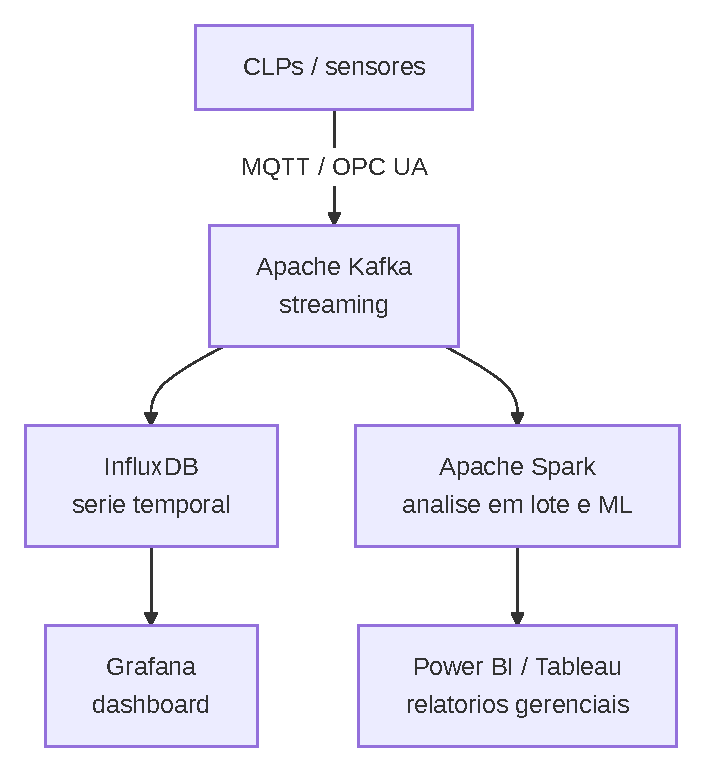
\includegraphics[width=\linewidth,height=0.8\textheight,keepaspectratio]{../figuras/capitulo-06-m2.pdf}%
}{\fbox{\parbox{0.9\linewidth}{\small Diagrama Mermaid ainda não renderizado: capitulo-06-m2. Rode scripts/render-mermaid.sh.}}}
\end{center}

\begin{caixafigura}

\textbf{{[}Figura 6.4 -- Stack de analytics industrial{]}}
\emph{Diagrama pipeline de dados: campo \ensuremath{\rightarrow} Kafka (streaming) \ensuremath{\rightarrow} InfluxDB (armazenamento) \ensuremath{\rightarrow} Grafana (visualização operacional) e \ensuremath{\rightarrow} Spark (processamento batch) \ensuremath{\rightarrow} BI (relatórios gerenciais). Ícones oficiais de cada ferramenta.}

\end{caixafigura}

\textbf{Apache Kafka:} plataforma de streaming distribuído --- ideal para processar fluxos de dados de centenas de equipamentos simultaneamente, com retenção configurável e tolerância a falhas.

\textbf{InfluxDB + Grafana:} a dupla open-source mais popular para monitoramento industrial. O InfluxDB armazena séries temporais com compressão eficiente; o Grafana exibe dashboards interativos com alertas.

\hypertarget{machine-learning-aplicado-uxe0-induxfastria}{%
\subsection{Machine Learning Aplicado à Indústria}\label{machine-learning-aplicado-uxe0-induxfastria}}

\begin{longtable}[]{@{}
  >{\raggedright\arraybackslash}p{(\columnwidth - 4\tabcolsep) * \real{0.3333}}
  >{\raggedright\arraybackslash}p{(\columnwidth - 4\tabcolsep) * \real{0.3333}}
  >{\raggedright\arraybackslash}p{(\columnwidth - 4\tabcolsep) * \real{0.3333}}@{}}
\toprule\noalign{}
\begin{minipage}[b]{\linewidth}\raggedright
Aplicação
\end{minipage} & \begin{minipage}[b]{\linewidth}\raggedright
Técnica de ML
\end{minipage} & \begin{minipage}[b]{\linewidth}\raggedright
Ferramenta
\end{minipage} \\
\midrule\noalign{}
\endhead
\bottomrule\noalign{}
\endlastfoot
Manutenção preditiva & Classificação, anomalia (Isolation Forest, LSTM) & AWS SageMaker, Azure ML, Python/scikit-learn \\
Otimização de processo & Regressão, otimização bayesiana & Aspen GDOT, TIBCO Spotfire \\
Visão computacional (qualidade) & CNN (VGG, ResNet, YOLO) & NVIDIA Jetson + TensorRT \\
Detecção de intrusão (cibersegurança) & Anomalia de rede, clustering & Darktrace, Claroty \\
\end{longtable}

\begin{caixaatencao}

\textbf{Atenção:} Modelos de ML para uso industrial devem ser \textbf{explicáveis} (\emph{Explainable AI}). Um operador precisa entender por que o sistema recomendou uma ação --- não pode confiar cegamente em uma ``caixa-preta'' em decisões que afetam segurança.

\end{caixaatencao}

\begin{center}\rule{0.5\linewidth}{0.5pt}\end{center}

\hypertarget{estudo-de-caso-iiot-em-planta-de-celulose}{%
\section{\texorpdfstring{Estudo de Caso --- IIoT em Planta de Celulose}{Estudo de Caso  IIoT em Planta de Celulose}}\label{estudo-de-caso-iiot-em-planta-de-celulose}}

\textbf{Contexto:} Uma fábrica de celulose no Brasil desejava reduzir as paradas não programadas de seus digestores (equipamentos críticos que operam a 170\ensuremath{^\circ}C e 8 bar).

\textbf{Solução implementada:}

\begin{enumerate}
\def\labelenumi{\arabic{enumi}.}
\tightlist
\item
  \textbf{Sensores adicionais:} acelerômetros em rolamentos das bombas de circulação + sensores de vibração nos agitadores dos digestores.
\item
  \textbf{Edge gateway:} coletou dados de vibração a 1 kHz; calculou localmente FFT (análise espectral) e transmitiu apenas os indicadores de frequência (não os dados brutos).
\item
  \textbf{Plataforma IIoT:} Azure IoT Hub recebeu os indicadores; modelo LSTM detectou padrões precursores de falha.
\item
  \textbf{Integração SCADA:} o modelo enviava alertas ao sistema SCADA (AVEVA System Platform) com antecedência de 72--120 horas antes da falha.
\end{enumerate}

\textbf{Resultados:} redução de 68\% nas paradas não programadas dos digestores; ROI atingido em 11 meses.

\begin{caixafigura}

\textbf{{[}Figura 6.5 -- Arquitetura IIoT da planta de celulose{]}}
\emph{Diagrama completo do estudo de caso: digestores com sensores de vibração \ensuremath{\rightarrow} edge gateway com FFT \ensuremath{\rightarrow} Azure IoT Hub \ensuremath{\rightarrow} modelo LSTM \ensuremath{\rightarrow} alerta no SCADA. Fotos ou ilustrações dos digestores industriais. Timeline mostrando detecção antecipada vs.~falha real.}

\end{caixafigura}

\begin{center}\rule{0.5\linewidth}{0.5pt}\end{center}

\hypertarget{resumo}{%
\section{Resumo}\label{resumo}}

\begin{itemize}
\tightlist
\item
  O \textbf{IIoT} aplica o paradigma IoT à indústria com requisitos rigorosos de confiabilidade, latência e segurança.
\item
  A arquitetura IIoT divide-se em três camadas: \textbf{Edge} (campo), \textbf{Fog} (intermediária) e \textbf{Cloud} (análise e gestão).
\item
  O \textbf{Edge Computing} é essencial para controle em tempo real, redução de banda e operação offline.
\item
  O \textbf{Digital Twin} permite simulação, otimização e manutenção preditiva sem risco à planta real.
\item
  A stack de analytics industrial (Kafka + InfluxDB + Grafana) democratizou o acesso a ferramentas de Big Data para o setor industrial.
\end{itemize}

\begin{center}\rule{0.5\linewidth}{0.5pt}\end{center}

\hypertarget{questuxf5es-de-revisuxe3o}{%
\section{Questões de Revisão}\label{questuxf5es-de-revisuxe3o}}

\textbf{Conceituais:}

\begin{enumerate}
\def\labelenumi{\arabic{enumi}.}
\tightlist
\item
  Cite três diferenças fundamentais entre IoT consumidor e IIoT industrial.
\item
  O que é Edge Computing? Por que processar dados na borda é vantajoso em aplicações industriais?
\item
  Explique o conceito de Digital Twin. Quais são os quatro tipos de Digital Twin descritos neste capítulo?
\end{enumerate}

\textbf{Práticas:}

\begin{enumerate}
\def\labelenumi{\arabic{enumi}.}
\setcounter{enumi}{3}
\tightlist
\item
  Uma empresa de mineração deseja monitorar remotamente 50 correias transportadoras, coletando vibração, temperatura de rolamentos e corrente dos motores. Proponha uma arquitetura IIoT com as camadas Edge, Fog e Cloud, especificando protocolos e ferramentas em cada camada.
\item
  Uma fábrica coleta 200 variáveis a cada segundo de um CLP. Calcule o volume de dados diário (em GB) sem compressão (assumindo float32 = 4 bytes por variável). Justifique por que o processamento na borda e a compressão de séries temporais são essenciais.
\end{enumerate}

\textbf{Desafio:}

\begin{enumerate}
\def\labelenumi{\arabic{enumi}.}
\setcounter{enumi}{5}
\tightlist
\item
  Elabore um projeto conceitual de Digital Twin para uma estação de bombeamento de água. Descreva: quais variáveis seriam sincronizadas, que modelo físico seria utilizado, como o twin poderia prever falhas e como ele se integraria ao SCADA existente.
\end{enumerate}

\begin{center}\rule{0.5\linewidth}{0.5pt}\end{center}

\hypertarget{referuxeancias}{%
\section{Referências}\label{referuxeancias}}

\begin{itemize}
\tightlist
\item
  IIC (Industrial Internet Consortium). \emph{Industrial Internet Reference Architecture (IIRA)}. IIC, 2019.
\item
  MICROSOFT. \emph{Azure IoT Reference Architecture}. Disponível em: \url{docs.microsoft.com/azure/architecture}.
\item
  AMAZON. \emph{AWS IoT Core Documentation}. Disponível em: \url{docs.aws.amazon.com/iot}.
\item
  GRIEVES, M. \emph{Digital Twin: Manufacturing Excellence through Virtual Factory Replication}. White Paper, 2014.
\item
  INFLUXDATA. \emph{InfluxDB and Grafana for Industrial IoT}. Disponível em: influxdata.com.
\end{itemize}
